\section{Kapitel 3}
\subsection{Teilaufgabe 1}
\subsubsection{Aufgabenstellung}
In der ersten Teilaufgabe sollten wir uns mit der Typkonvertierung befassen. Dafür schreiben wir
ein kleines Programm, welches die primitiven Datentypen erweiternd und einschränkend
Konvertiert.

\subsubsection{Anforderungsdefinition}
\begin{enumerate}
	\item Zu jedem Primitiven Datentypen eine erweiternde und einschränkende Konvertierung
	durchführen.
\end{enumerate}

\subsubsection{Entwurf}
\begin{center}
	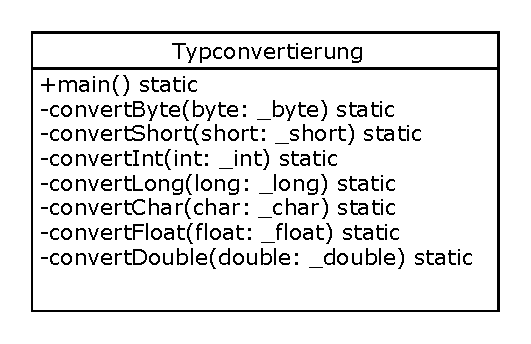
\includegraphics[width=0.6\textwidth]{uml/uml_c3_p1.pdf}
\end{center}

\subsubsection{Quelltext}
\paragraph{Typkonvertierungen.java}\
\lstinputlisting[language = Java , frame = trBL , escapeinside={(*@}{@*)}]{../chapter_03/src/main/java/chapter_03/Typkonvertierungen.java}

\subsubsection{Testdokumentation}
Nach den Aufruf des Programms, sollten alle Typkonvertierungen auf der Konsole ausgegeben
werden. Dies ist auch geschehen.

\subsubsection{Benutzungshinweise}
Keine Besonderen Benutzungshinweise.
Man navigiere zu dem Ordner von sich die Compilierte Datei mit dem Namen "Typkonvertierungen.class"
\space befindet und führt anschlie\ss end java Typkonvertierungen aus.

\subsubsection{Anwendungsbeispiel}
Nach dem man das Programm gestartet hat (aufgrund der Formatierung, werden einige Zeichen bei Char nicht dargestellt), sollte folgende Ausgabe erscheinen:

\begin{lstlisting}[frame = trBL , escapeinside={(*@}{@*)}]
[sebastian@laptop bin]$ java Typkonvertierungen
---------------------
Byte erweiternd
Byte   -128
Short  -128
Int    -128
Long   -128
Float  -128.0
Double -128.0

Char   タ
---------------------
Short einschränkend
Short  34
Byte   34
Short erweiternd
Short  34
Int    34
Long   34
Float  34.0
Double 34.0

Char   "
---------------------
Int einschränkend
Int    98987
Short  -32085
Byte   -85
Int erweiternd
Int    98987
Long   98987
Float  98987.0
Double 98987.0

Char   芫
---------------------
Long einschränkend
Long   987987987
Int    987987987
Short  -32749
Byte   19
Long erweiternd
Long   987987987
Float  9.8798797E8
Double 9.87987987E8

Char   耓
---------------------
Char einschränkend
Char   a
Long   97
Int    97
Short  97
Byte   97
Char erweiternd
Char   a
Long   97
Float  97.0
Double 97.0
---------------------
Float einschränkend
Float  15.0
Long   15
Int    15
Short  15
Byte   15
Float erweiternd
Float  15.0
Double 15.0

Char   
---------------------
Double einschränkend
Double 1.7976931348623157E308
Float  Infinity
Long   9223372036854775807
Int    2147483647
Short  -1
Byte   -1

Char   ￿
---------------------
[sebastian@laptop bin]$ 
\end{lstlisting}
